\centering

\begin{minipage}[t]{\textwidth}
\centering
\scalebox{0.76}{
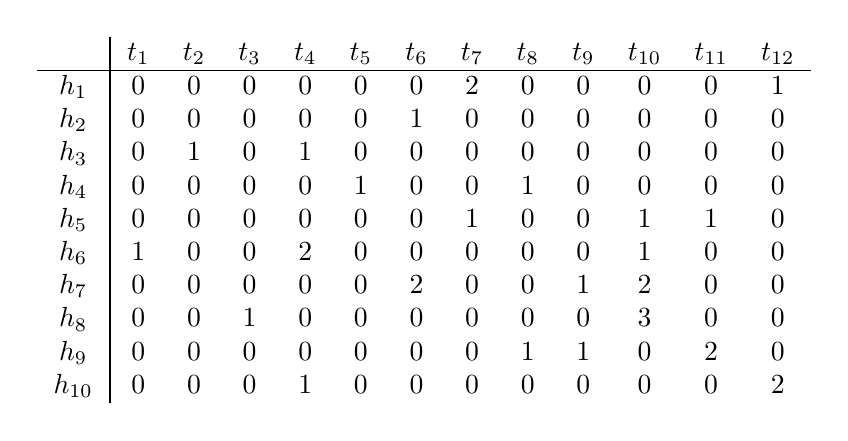
\begin{tikzpicture}[
    node distance=1cm,
    test/.style={circle, draw, thick, minimum size=0.6cm},
    decision/.style={circle, draw, thick, minimum size=0.55cm},
    leaf/.style={circle, draw, thick, fill=green!20, minimum size=0.5cm},
    arrow/.style={->, thick}
]

% Table of hypotheses vs tests (10 hypotheses, 12 tests, unbalanced outcomes)
\node[] at (0,0) {
\begin{tabular}{c|cccccccccccc}
 & $t_1$ & $t_2$ & $t_3$ & $t_4$ & $t_5$ & $t_6$ & $t_7$ & $t_8$ & $t_9$ & $t_{10}$ & $t_{11}$ & $t_{12}$ \\
\hline
$h_1$ & 0 & 0 & 0 & 0 & 0 & 0 & 2 & 0 & 0 & 0 & 0 & 1 \\
$h_2$ & 0 & 0 & 0 & 0 & 0 & 1 & 0 & 0 & 0 & 0 & 0 & 0 \\
$h_3$ & 0 & 1 & 0 & 1 & 0 & 0 & 0 & 0 & 0 & 0 & 0 & 0 \\
$h_4$ & 0 & 0 & 0 & 0 & 1 & 0 & 0 & 1 & 0 & 0 & 0 & 0 \\
$h_5$ & 0 & 0 & 0 & 0 & 0 & 0 & 1 & 0 & 0 & 1 & 1 & 0 \\
$h_6$ & 1 & 0 & 0 & 2 & 0 & 0 & 0 & 0 & 0 & 1 & 0 & 0 \\
$h_7$ & 0 & 0 & 0 & 0 & 0 & 2 & 0 & 0 & 1 & 2 & 0 & 0 \\
$h_8$ & 0 & 0 & 1 & 0 & 0 & 0 & 0 & 0 & 0 & 3 & 0 & 0 \\
$h_9$ & 0 & 0 & 0 & 0 & 0 & 0 & 0 & 1 & 1 & 0 & 2 & 0 \\
$h_{10}$ & 0 & 0 & 0 & 1 & 0 & 0 & 0 & 0 & 0 & 0 & 0 & 2 \\
\end{tabular}
};

\end{tikzpicture}
}
\normalsize
\caption*{(a) Hypotheses and tests table}
\end{minipage}

\begin{minipage}[t]{0.43\textwidth}
\centering
\scalebox{0.78}{
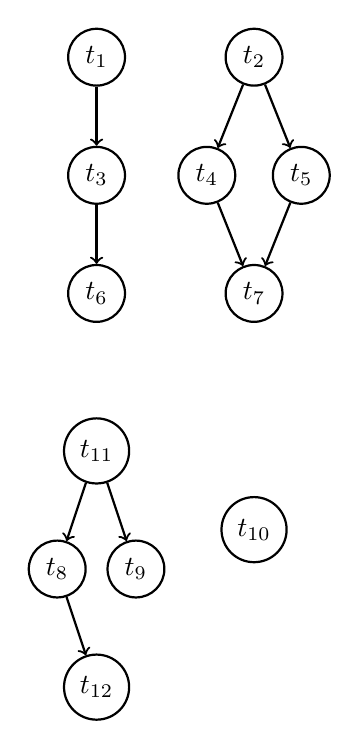
\begin{tikzpicture}[
    node distance=1cm,
    test/.style={circle, draw, thick, minimum size=0.6cm},
    arrow/.style={->, thick}
]

% DAG with 4 components (2 components on top, 2 below)
% Component 1 (top left)
\node[test] (t1) at (0.5,0) {$t_1$};
\node[test] (t3) at (0.5,-1.5) {$t_3$};
\node[test] (t6) at (0.5,-3) {$t_6$};
\draw[arrow] (t1) -- (t3);
\draw[arrow] (t3) -- (t6);

% Component 2 (top right)
\node[test] (t2) at (2.5,0) {$t_2$};
\node[test] (t4) at (1.9,-1.5) {$t_4$};
\node[test] (t5) at (3.1,-1.5) {$t_5$};
\node[test] (t7) at (2.5,-3) {$t_7$};
\draw[arrow] (t2) -- (t4);
\draw[arrow] (t2) -- (t5);
\draw[arrow] (t4) -- (t7);
\draw[arrow] (t5) -- (t7);

% Component 3 (bottom left)
\node[test] (t11) at (0.5,-5) {$t_{11}$};
\node[test] (t8) at (0,-6.5) {$t_8$};
\node[test] (t9) at (1,-6.5) {$t_9$};
\node[test] (t12) at (0.5,-8) {$t_{12}$};
\draw[arrow] (t11) -- (t8);
\draw[arrow] (t11) -- (t9);
\draw[arrow] (t8) -- (t12);

% Component 4 (isolated node, bottom right)
\node[test] (t10) at (2.5,-6) {$t_{10}$};

\end{tikzpicture}
}
\normalsize
\caption*{(b) Precedence}
\end{minipage}
\hfill
\begin{minipage}[t]{0.55\textwidth}
\centering
\scalebox{0.78}{
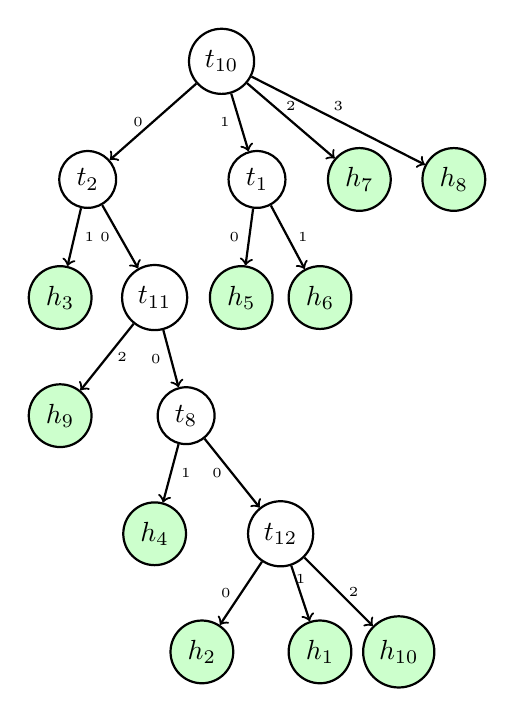
\begin{tikzpicture}[
    node distance=1cm,
    decision/.style={circle, draw, thick, minimum size=0.55cm},
    leaf/.style={circle, draw, thick, fill=green!20, minimum size=0.5cm},
    arrow/.style={->, thick}
]

% Decision tree built from table analysis
% Root: t10 (separates: h5→1, h6→1, h7→2, h8→3, rest→0)
\node[decision] (root) at (4.25,0) {$t_{10}$};

% t10=0: {h1,h2,h3,h4,h9,h10}
\node[decision] (n1) at (2.55,-1.5) {$t_2$};
% t10=1: {h5,h6}
\node[decision] (n2) at (4.7,-1.5) {$t_1$};
% t10=2: {h7}
\node[leaf] (h7) at (6,-1.5) {$h_7$};
% t10=3: {h8}
\node[leaf] (h8) at (7.2,-1.5) {$h_8$};

% t10=0, t2=0: {h1,h2,h4,h9,h10}
\node[decision] (n3) at (3.4,-3) {$t_{11}$};
% t10=0, t2=1: {h3}
\node[leaf] (h3) at (2.2,-3) {$h_3$};

% t10=1, t1=0: {h5}
\node[leaf] (h5) at (4.5,-3) {$h_5$};
% t10=1, t1=1: {h6}
\node[leaf] (h6) at (5.5,-3) {$h_6$};

% t10=0, t2=0, t11=0: {h1,h2,h4,h10}
\node[decision] (n4) at (3.8,-4.5) {$t_8$};
% t10=0, t2=0, t11=1: {h5} - but h5 already separated
% t10=0, t2=0, t11=2: {h9}
\node[leaf] (h9) at (2.2,-4.5) {$h_9$};

% t10=0, t2=0, t11=0, t8=0: {h1,h2,h10}
\node[decision] (n5) at (5,-6) {$t_{12}$};
% t10=0, t2=0, t11=0, t8=1: {h4}
\node[leaf] (h4) at (3.4,-6) {$h_4$};

% t10=0, t2=0, t11=0, t8=0, t12=0: {h2}
\node[leaf] (h2) at (4,-7.5) {$h_2$};
% t10=0, t2=0, t11=0, t8=0, t12=1: {h1}
\node[leaf] (h1) at (5.5,-7.5) {$h_1$};
% t10=0, t2=0, t11=0, t8=0, t12=2: {h10}
\node[leaf] (h10) at (6.5,-7.5) {$h_{10}$};

% Edges
\draw[arrow] (root) -- (n1) node[midway, left, font=\tiny] {0};
\draw[arrow] (root) -- (n2) node[midway, left, font=\tiny] {1};
\draw[arrow] (root) -- (h7) node[midway, above, font=\tiny] {2};
\draw[arrow] (root) -- (h8) node[midway, above, font=\tiny] {3};

\draw[arrow] (n1) -- (n3) node[midway, left, font=\tiny] {0};
\draw[arrow] (n1) -- (h3) node[midway, right, font=\tiny] {1};

\draw[arrow] (n2) -- (h5) node[midway, left, font=\tiny] {0};
\draw[arrow] (n2) -- (h6) node[midway, right, font=\tiny] {1};

\draw[arrow] (n3) -- (n4) node[midway, left, font=\tiny] {0};
\draw[arrow] (n3) -- (h9) node[midway, right, font=\tiny] {2};

\draw[arrow] (n4) -- (n5) node[midway, left, font=\tiny] {0};
\draw[arrow] (n4) -- (h4) node[midway, right, font=\tiny] {1};

\draw[arrow] (n5) -- (h2) node[midway, left, font=\tiny] {0};
\draw[arrow] (n5) -- (h1) node[midway, above, font=\tiny] {1};
\draw[arrow] (n5) -- (h10) node[midway, right, font=\tiny] {2};

\end{tikzpicture}
}
\normalsize
\caption*{(c) Valid decision tree}
\end{minipage}
